%! Author = Saeid Yazdani
%! Date = 9/8/2024


\section{Functional Tests}
\label{sec:functional-tests}

The system as a whole was evaluated with functional tests to verify that it
operates according to design specifications and performs the intended functions:

\begin{itemize}[topsep=8pt,itemsep=4pt,partopsep=4pt, parsep=4pt]
    \item \textbf{Firmware/Software Integration:}
    ensures that the software controlling the hardware is working properly,
    and safety guards are engaging correctly.

    \item \textbf{Signal and Data Flow Validation:}
    Verify that inputs result in correct outputs, communication protocol is
    working properly, and relays and sensors are responding as expected.

    \item \textbf{Real-World Scenarios:}
    Simulating real-world operational conditions, including testing at
    different voltages, temperatures, loads and stability in extended
    operation times.

\end{itemize}

Multiple instruments
are used for the calibration of voltage and current values and for
cross-measuring system's input and output for functional validation.
\autoref{fig:hvs-development-rack} shows the development rack and the supporting
equipment.

\begin{figure}[p]
    \centering
    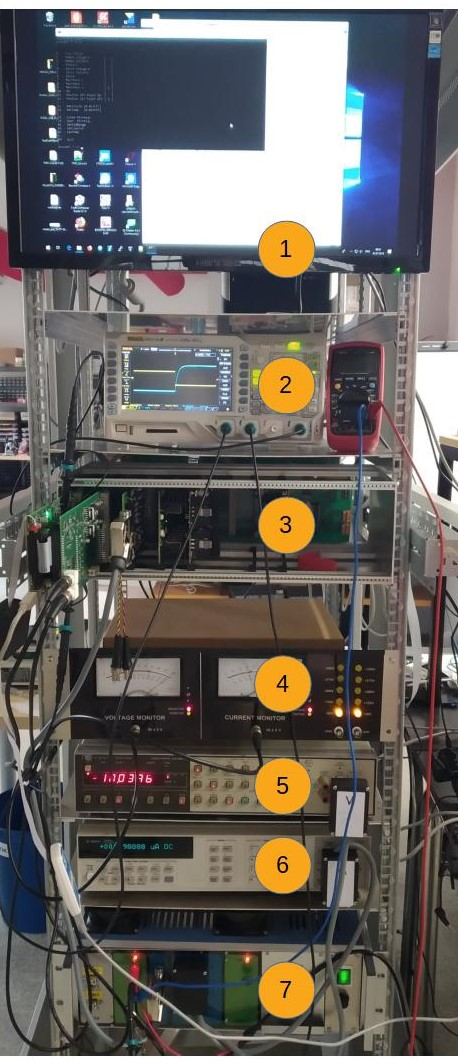
\includegraphics[width=\linewidth,height=0.85\textheight,keepaspectratio]
    {figures/prototype/production/image12}
    \caption[System Test Rack]{
        The \acs{HVS} system test and development tower.
        \textbf{(1)} A PC for executing the operator software.
        \textbf{(2)} Oscilloscope for signal debugging.
        \textbf{(3)} The \ac{HVS}.
        \textbf{(4)} Analog meters connected to the monitor board.
        \textbf{(5)} Multimeter for voltage measurements.
        \textbf{(6)} Multimeter for current measurements.
        \textbf{(7)} Custom-made array of switchable resistive loads.
    }
    \label{fig:hvs-development-rack}
\end{figure}

\subsection{Full-Swing Tests}
\label{subsec:full-swing-tests}

% 600V Swing
\autoref{fig:640v_swing_no_compensation} shows the \acs{HVS} response to
a full-range \SI{\pm320}{\volt}
swing from the negative to the positive quadrant without any compensation.
The transition from \SI{-300}{\volt} to \SI{+300}{\volt} has a settling time of
\SI{250}{\micro\second} and slight overshoot of \SI{25}{\volt} which is a
remarkable and on par with premium high-voltage power supplies in the market.

\begin{figure}[htbp]
    \centering
    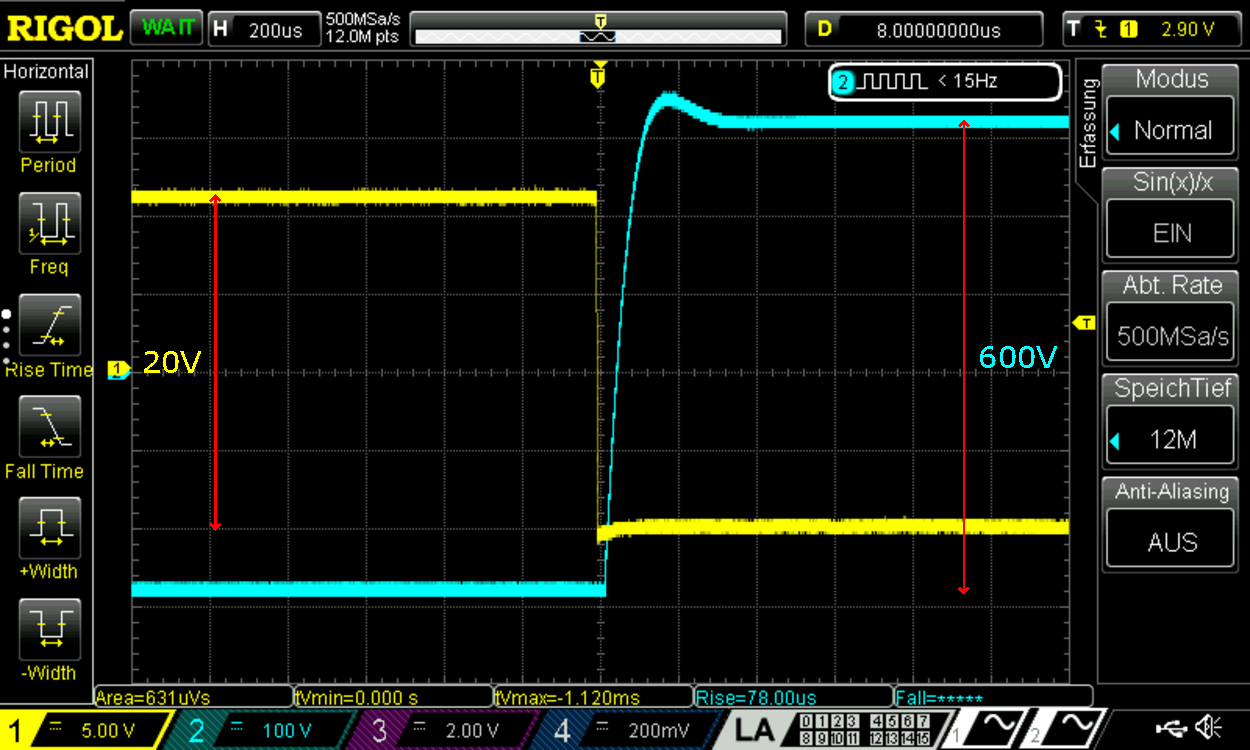
\includegraphics[width=\textwidth]
    {figures/tests/640v_swing_no_compensation}
    \caption[\SI{\pm300}{\volt} Swing Test With No Compensation]{
        Without dynamic compensation, the \acs{HVS} achieved a
        full range swing of \SI{600}{\volt}, settling time of
        \SI{250}{\micro\second} and slight overshoot of \SI{20}{\volt}.
        The control signal is inverted.
        \textbf{Blue Signal:} \acs{HVS} Output (\SI{100}{\volt} per division).
        \textbf{Yellow Signal:} Pre Amplifier output (\SI{5}{\volt} per division).
        \SI{200}{\micro\second} Timebase.
    }
    \label{fig:640v_swing_no_compensation}
\end{figure}

\begin{figure}[htbp]
    \centering
    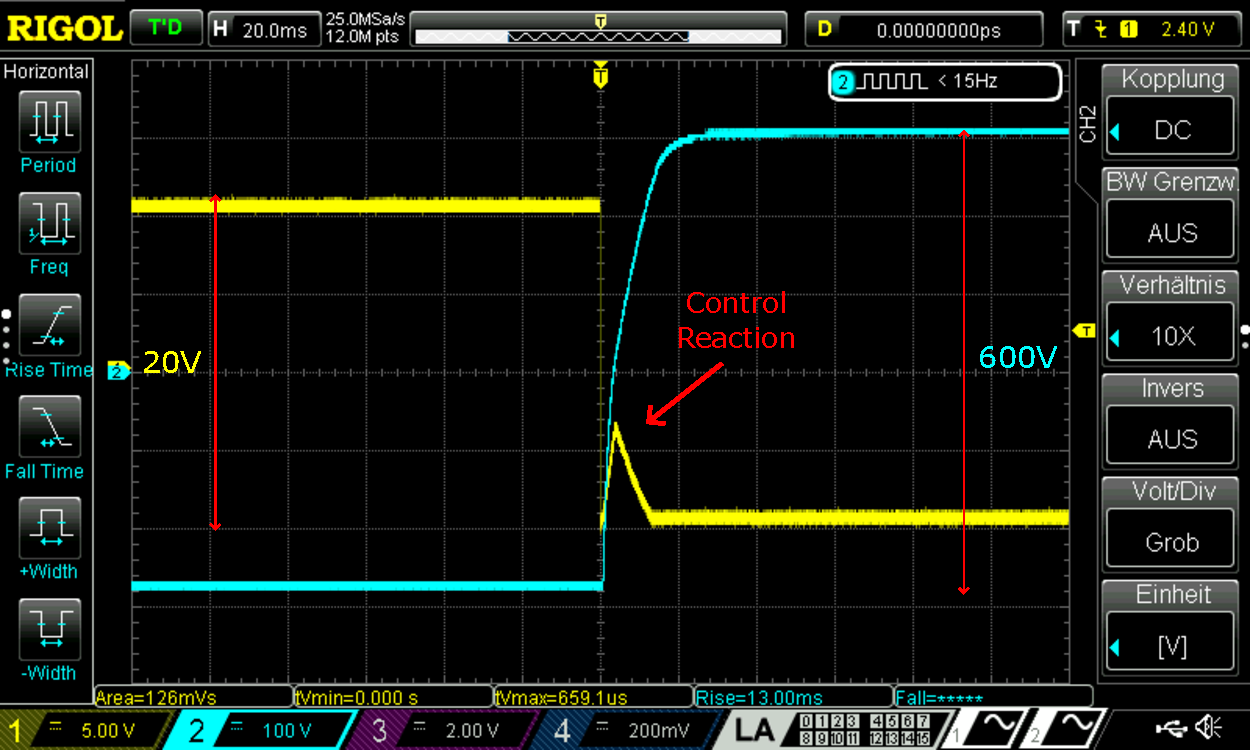
\includegraphics[width=\textwidth]
    {figures/tests/640v_swing_with_compensation}
    \caption[\SI{\pm320}{\volt} Swing Test With Dynamic Compensation]{
        By engaging the dynamic compensation, the \acs{HVS} achieved a
        swing of \SI{600}{\volt} and settling time of
        \SI{22}{\milli\second} without any \emph{overshoot}.
        The bounce visible on the pre amplifier signal issued by the FPGA
        compensates and suppresses the overshoot.
        \textbf{Blue Signal:} \acs{HVS} Output (\SI{100}{\volt} per division).
        \textbf{Yellow Signal:} Pre Amplifier output (\SI{5}{\volt} per division).
        \SI{20}{\milli\second} Timebase.
    }
    \label{fig:640v_swing_with_compensation}
\end{figure}

% With the application of dynamic compensation
% to adapt the power stage to the \ac{DUT}'s specific needs.
\autoref{fig:640v_swing_with_compensation} shows the same test setup but with
the dynamic compensation enabled.
This time, the overshoot is suppressed by the control loop where near the peak
of the voltage swing control signal performs the adjustments to prevent the
overshoot.
The achieved settling time in this mode is \SI{20}{\milli\second} that is
increased by a factor of 80.

% 20V swing
The result of a half-range swing test for the lower range of \SI{\pm10}{\volt}
with dynamic compensation enabled is shown in \autoref{fig:0Vto8V_swing_with_compensation}.
In this test, the voltage swings from \SI{-4}{\volt} to \SI{+4}{\volt}
with a settling time of \SI{4}{\milli\second} with no overshoot.

\begin{figure}[h!]
    \centering
    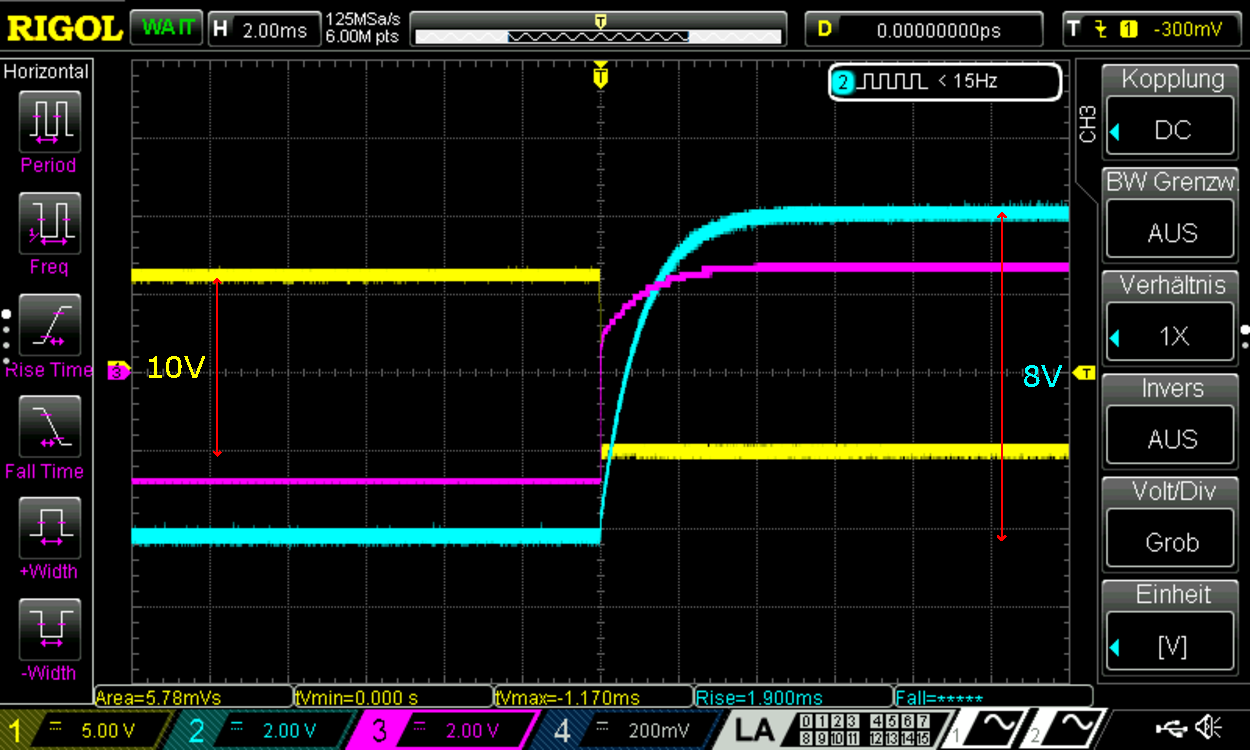
\includegraphics[width=\textwidth]
    {figures/tests/10v_positive_swing_with_compensation}
    \caption[\SI{\pm10}{\volt} Swing Test With Dynamic Compensation]{
        With dynamic compensation enabled, the \acs{HVS} manages to swing
        from \SI{-4}{\volt} to \SI{+4}{\volt} in \SI{4}{\milli\second}
        without any overshoot for a resistive load of \SI{75}{\ohm}.
        \textbf{Blue Signal:} \acs{HVS} Output (\SI{2}{\volt} per division).
        \textbf{Pink Signal:} Current Signal (\SI{50}{\milli\ampere} per division).
        \textbf{Yellow Signal:} Pre Amplifier output (\SI{5}{\volt} per division).
        \SI{2}{\milli\second} Timebase.
    }
    \label{fig:0Vto8V_swing_with_compensation}
\end{figure}

\subsection{Enduring Stability Test}
\label{subsec:longtime-stability-test}

To test the long-term stability of the \acs{HVS}, it was used as a constant
current source in a platform for testing the reliability of
\acs{PCB} traces and interconnects under harsh environments developed at
TU Chemnitz \autocite{9547972}.

In this test method, a power supply is required to force a constant current
with a minimum amount of deviation for a long period into a series
chain of traces with multiple vias on a large \acs{PCB}.
The test \acs{PCB} then is inserted in a thermal chamber and undergoes
temperature cycling in \SI{20}{\degreeCelsius} to \SI{140}{\degreeCelsius}
range.
A fixed current is necessary to measure changes in the resistance over a
typical period of one month or until a trace fails-open due to via barrel
crack or delamination. The test elements and their description are presented in
\autoref{fig:hvs-as-current-source-in-pcb-tester}.

\clearpage
The \acs{HVS} managed to effectively yield on par results with another
industry standard lab power supply over a period of two weeks until the
tests stopped.
Sample sof these measurement results are presented in
\autoref{fig:via-chain-results}.

\begin{figure}[ht]
    \centering

    % Top figure
    \begin{minipage}{\textwidth}
        \centering
        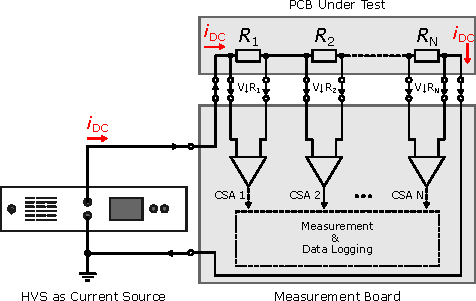
\includegraphics[width=0.75\textwidth]{figures/tests/via-chain-equivallent-circuit}
        \subcaption{Equivallend circuit of the \acs{PCB} reliability test method.
        }
        \label{fig:top}
    \end{minipage}

    % Space between figures
    \vspace{1em}

    % Two figures side by side
    \begin{minipage}{0.49\textwidth}
        \centering
        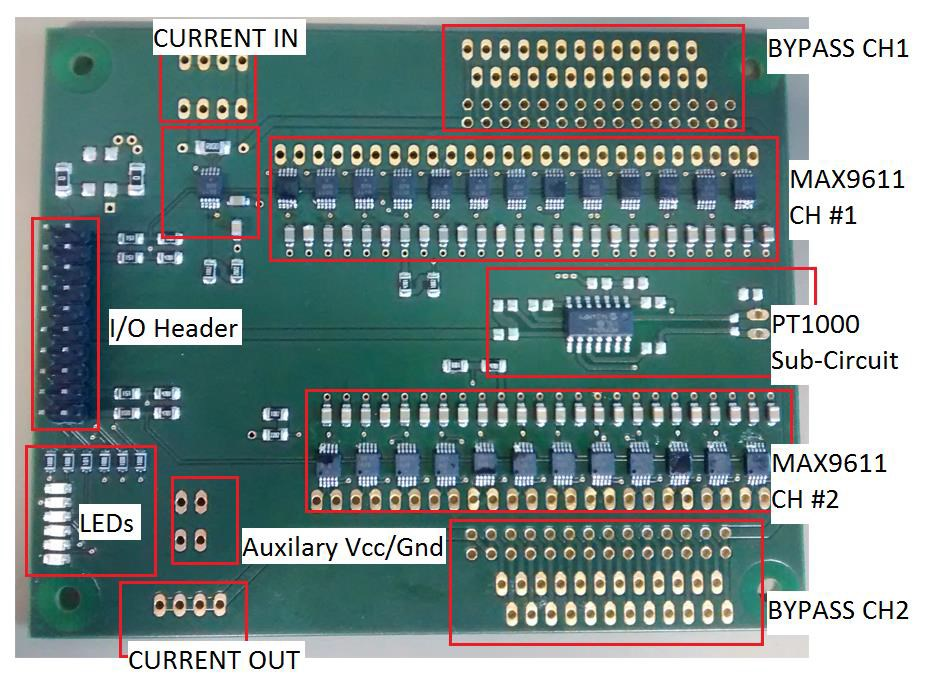
\includegraphics[width=\textwidth]{figures/tests/via-chain-measurement-board}
        \subcaption{Control board for wiring and data-logging.}
        \label{fig:bottomleft}
    \end{minipage}
    \hfill
    \begin{minipage}{0.49\textwidth}
        \centering
        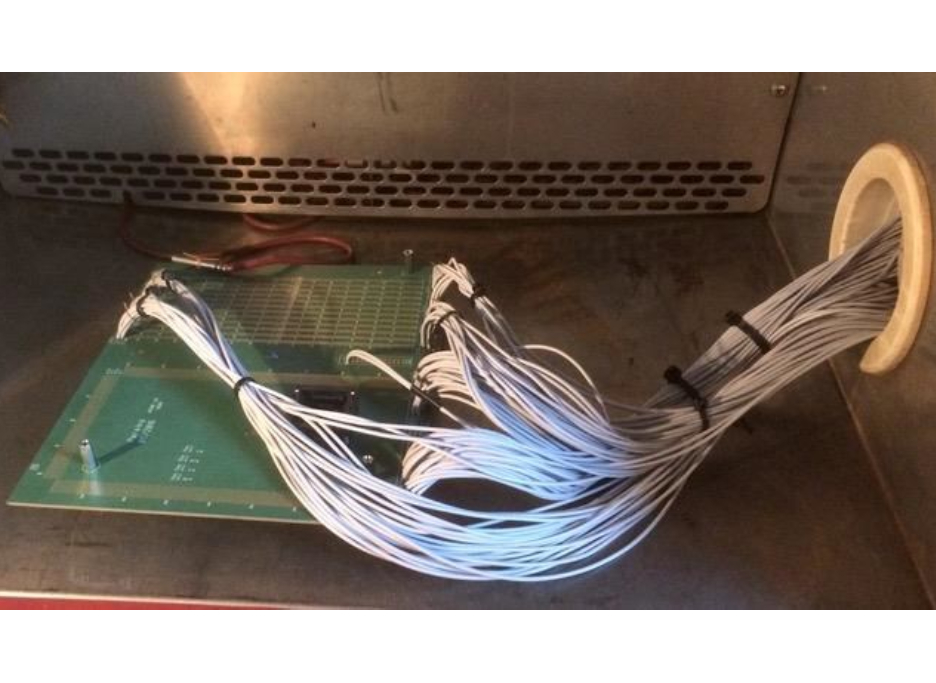
\includegraphics[width=\textwidth]{figures/tests/via-chain-in-oven}
        \subcaption{The \acs{PCB} test coupon inserted into a thermal chamber.
        }
        \label{fig:bottomright}
    \end{minipage}

    \caption[\acs{HVS} as Current Source in \acs{PCB} Reliability Test Platform]{
        A Constant current goes through each \acs{PCB} trace/interconnect on the
        test \acs{PCB}. These interconnects acts as a shunt resistor for their
        dedicated \ac{CSA}.
        Since the amount of current is known, the resulting voltage drop will
        yield the resistance of the interconnect under test.
        The changes in resistance at different temperatures will be recorded
        over time and deviations from the initial state will be studied.
    }
    \label{fig:hvs-as-current-source-in-pcb-tester}
\end{figure}

\begin{figure}[ht!]
    \centering
    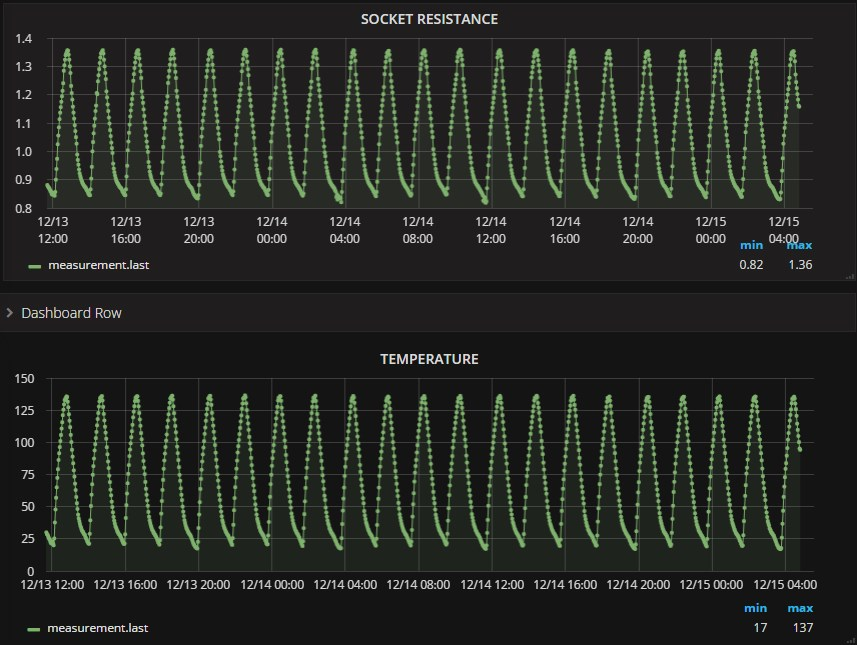
\includegraphics[width=0.8\textwidth]
    {figures/tests/via-chain-results}
    \caption[\acs{HVS} Long-Term Test Sample Result]{
        Measurement results of an interconnect on the test \acs{PCB} Under Test.
        Over two days the resistance of the interconnect has increased and
        decreased linearly against the temperature.
        The \acs{HVS} was used as a current source to apply a known stable current at
        fixed intervals for measuring the resistance according to the voltage drop
        over the interconnect.
    }
    \label{fig:via-chain-results}
\end{figure}
